\documentclass{scrartcl}
\usepackage{german}
\usepackage[T1]{fontenc}
\usepackage[latin1]{inputenc}
\usepackage[german]{babel}

% zusätzliche mathematische Symbole, AMS=American Mathematical Society
\usepackage{amssymb}

% fürs Einbinden von Graphiken
\usepackage{graphicx}

% für Namen etc. in Kopf- oder Fußzeile
\usepackage{fancyhdr}

% erlaubt benutzerdefinierte Kopfzeilen
\pagestyle{fancy}

% Definition der Kopfzeile
\lhead{
\begin{tabular}{ll}
Fisnik Zeqiri & 4306430 \\
Felix  Karg   & 4342014
\end{tabular}
}
\chead{}
\rhead{\today{}}
\lfoot{}
\cfoot{Seite \thepage}
\rfoot{}

\begin{document}
\section*{Antworten zum �bungsblatt Nr. 7}

\section*{Aufgabe 1}
\section*{Aufgabe 2}
\section*{Aufgabe 3}
\begin{itemize}
    \item[a)] [Schaltkreis 1] \\
	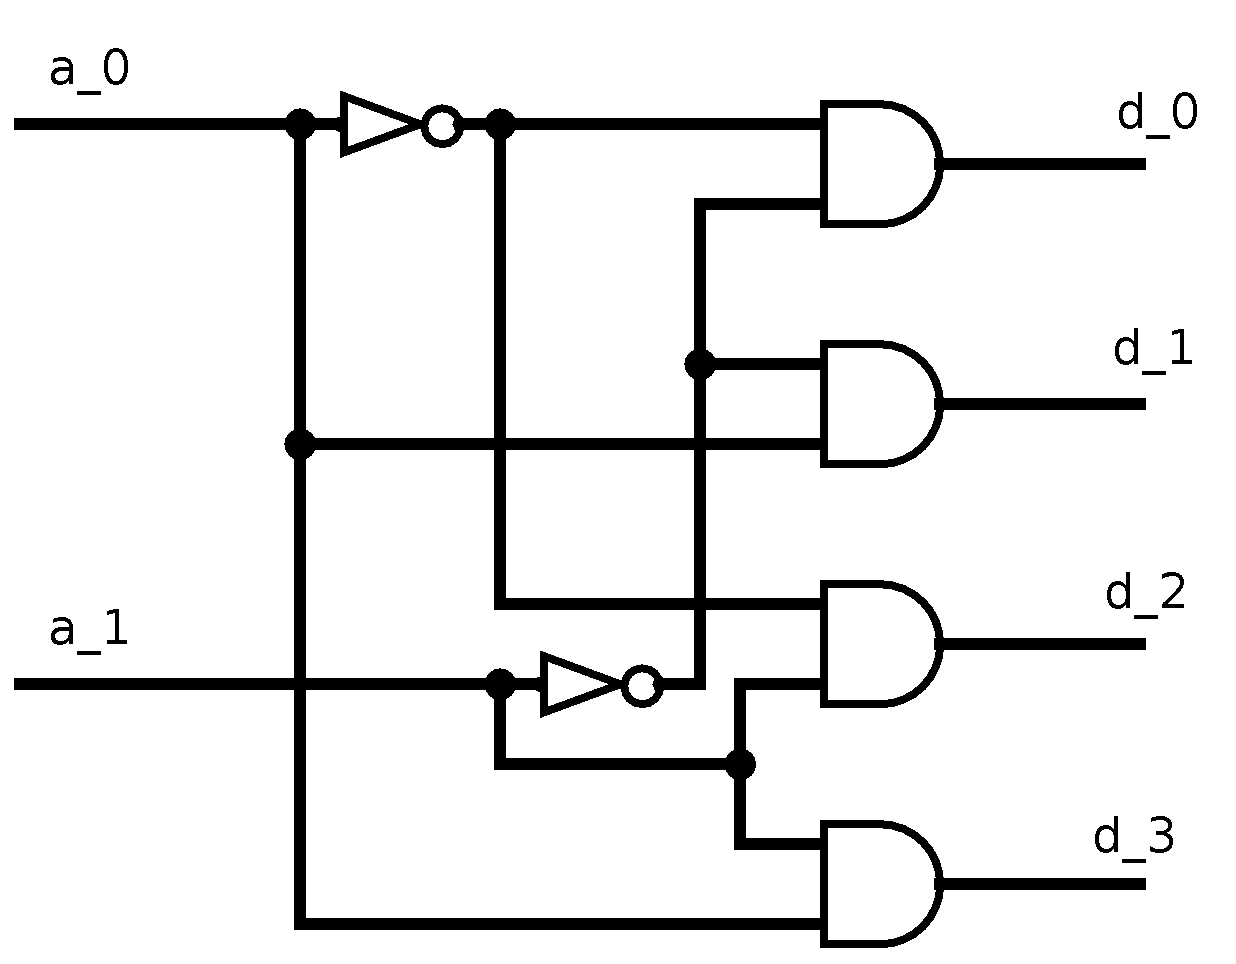
\includegraphics[width=13cm]{circuit_1.png}
    \item[b)] [Schaltkreis 2] \\
	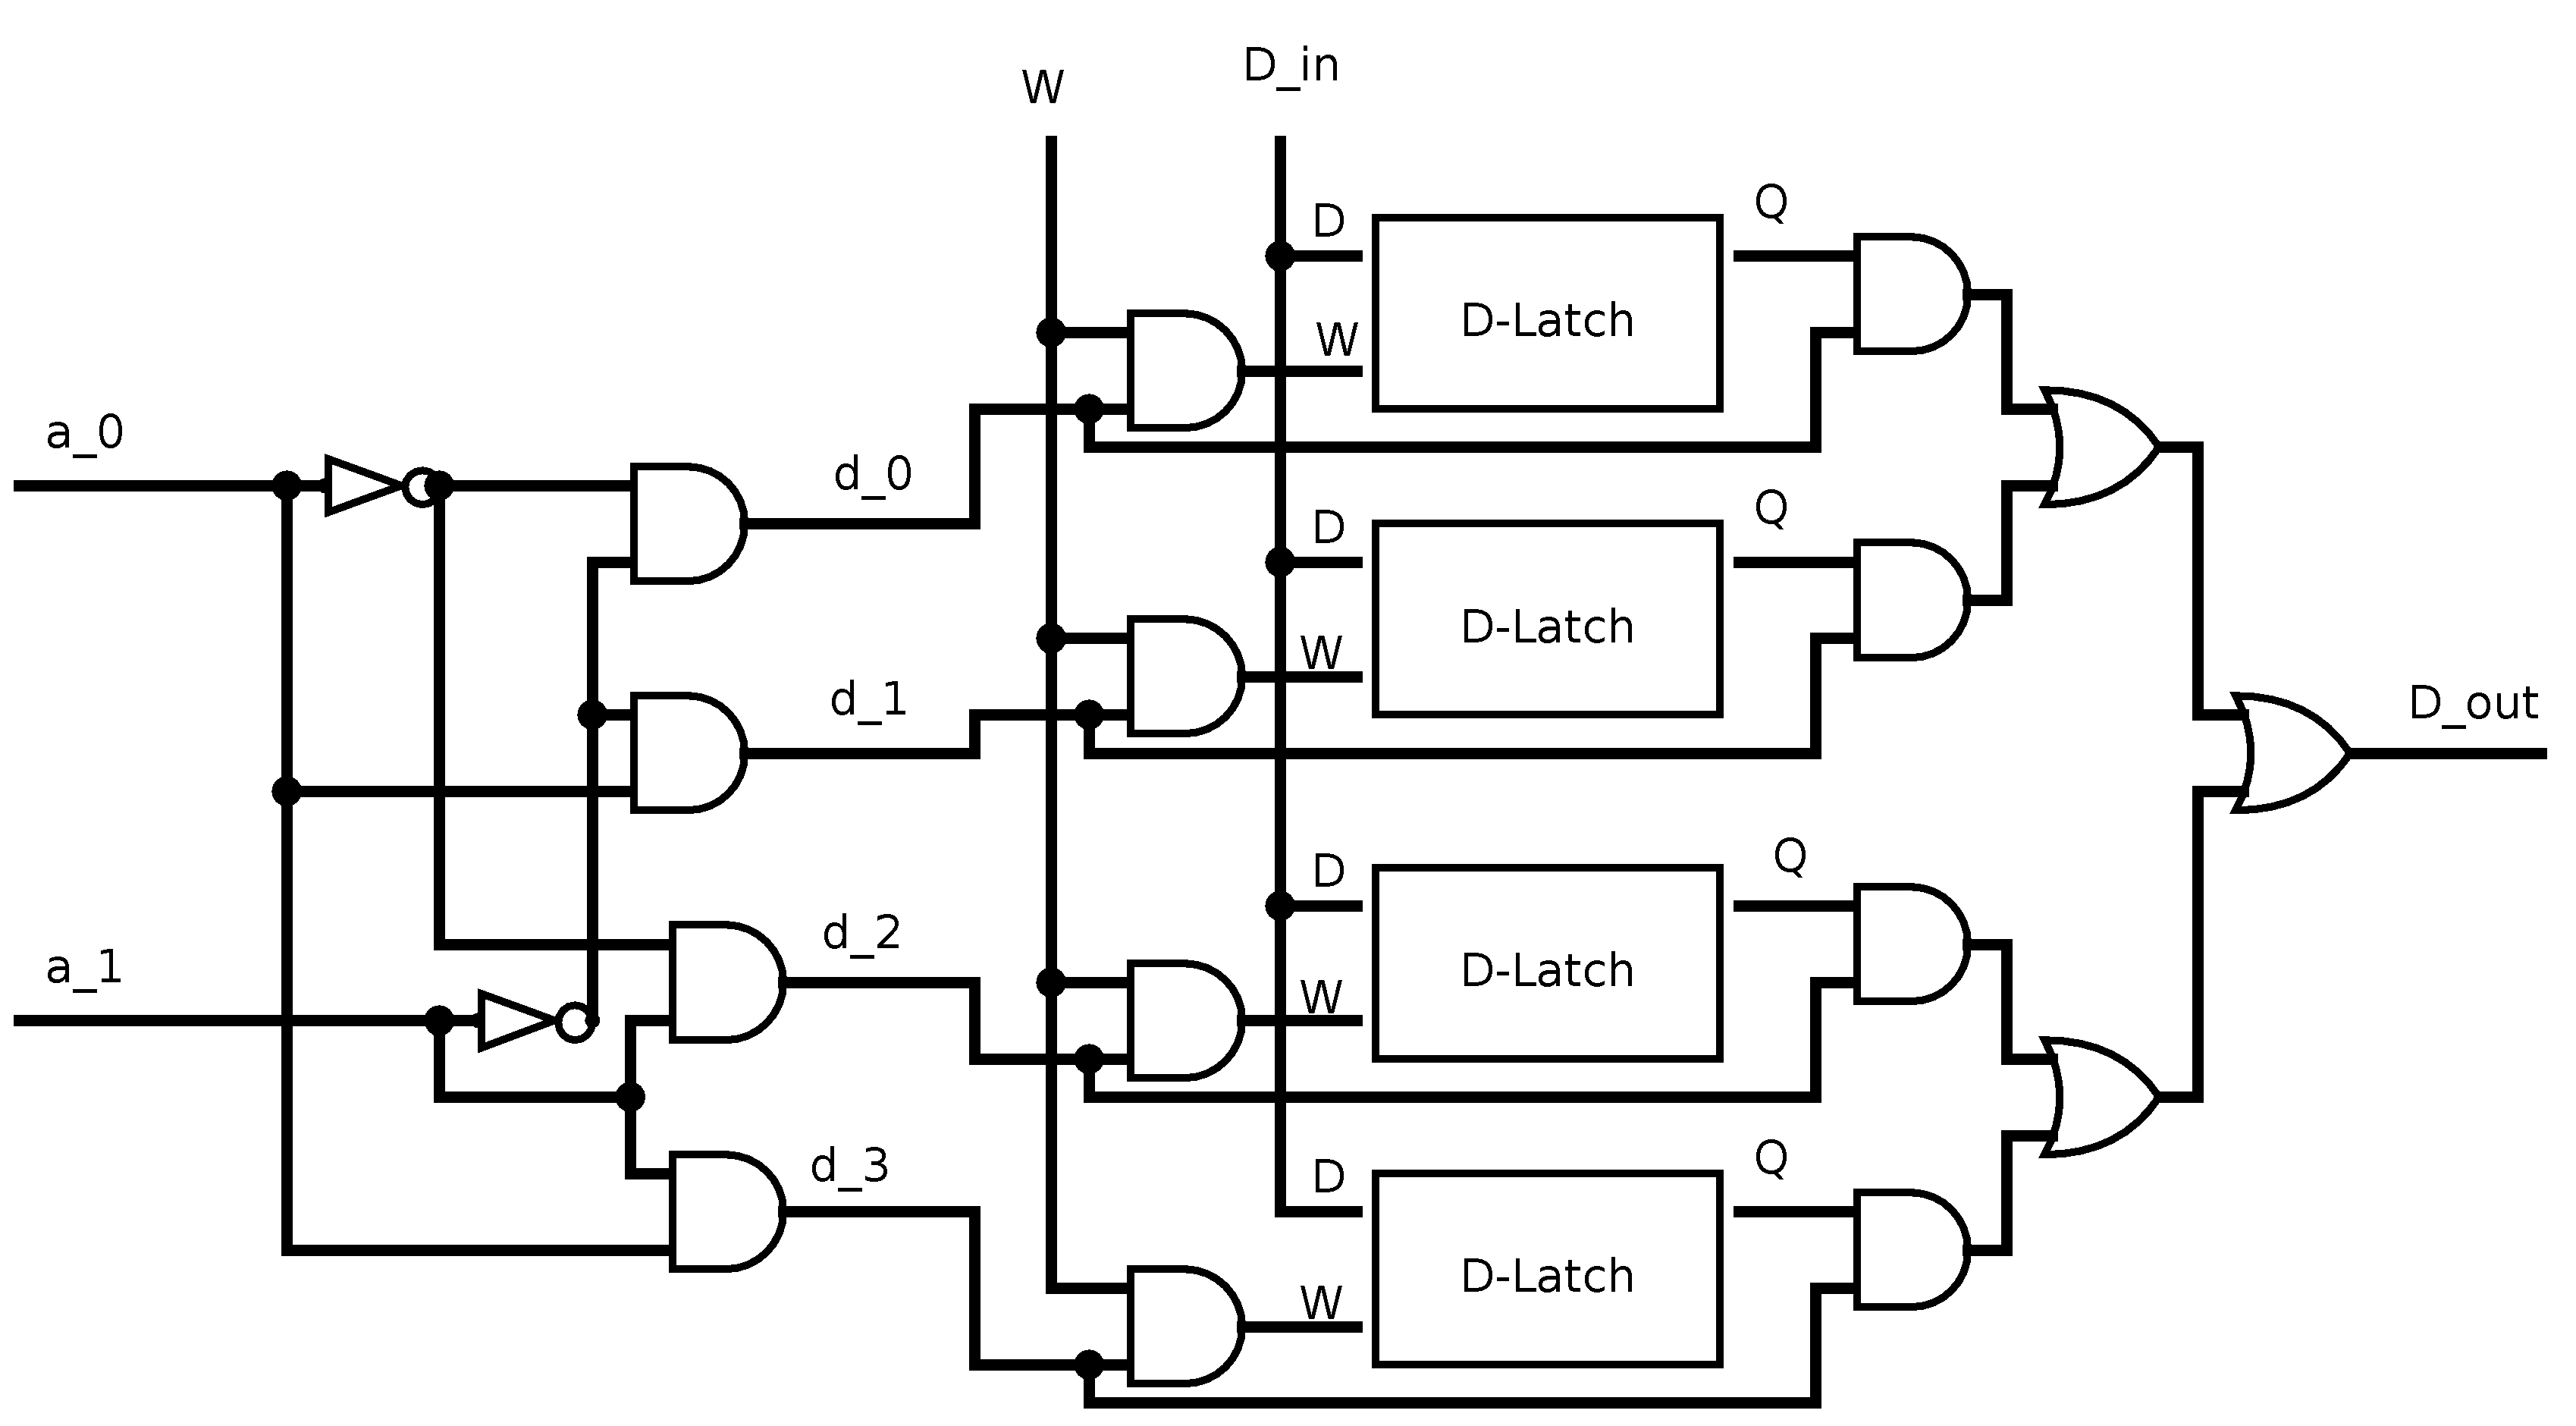
\includegraphics[width=14cm]{circuit_2.png}
    \item[c)] [Schaltkreis 3] \\
	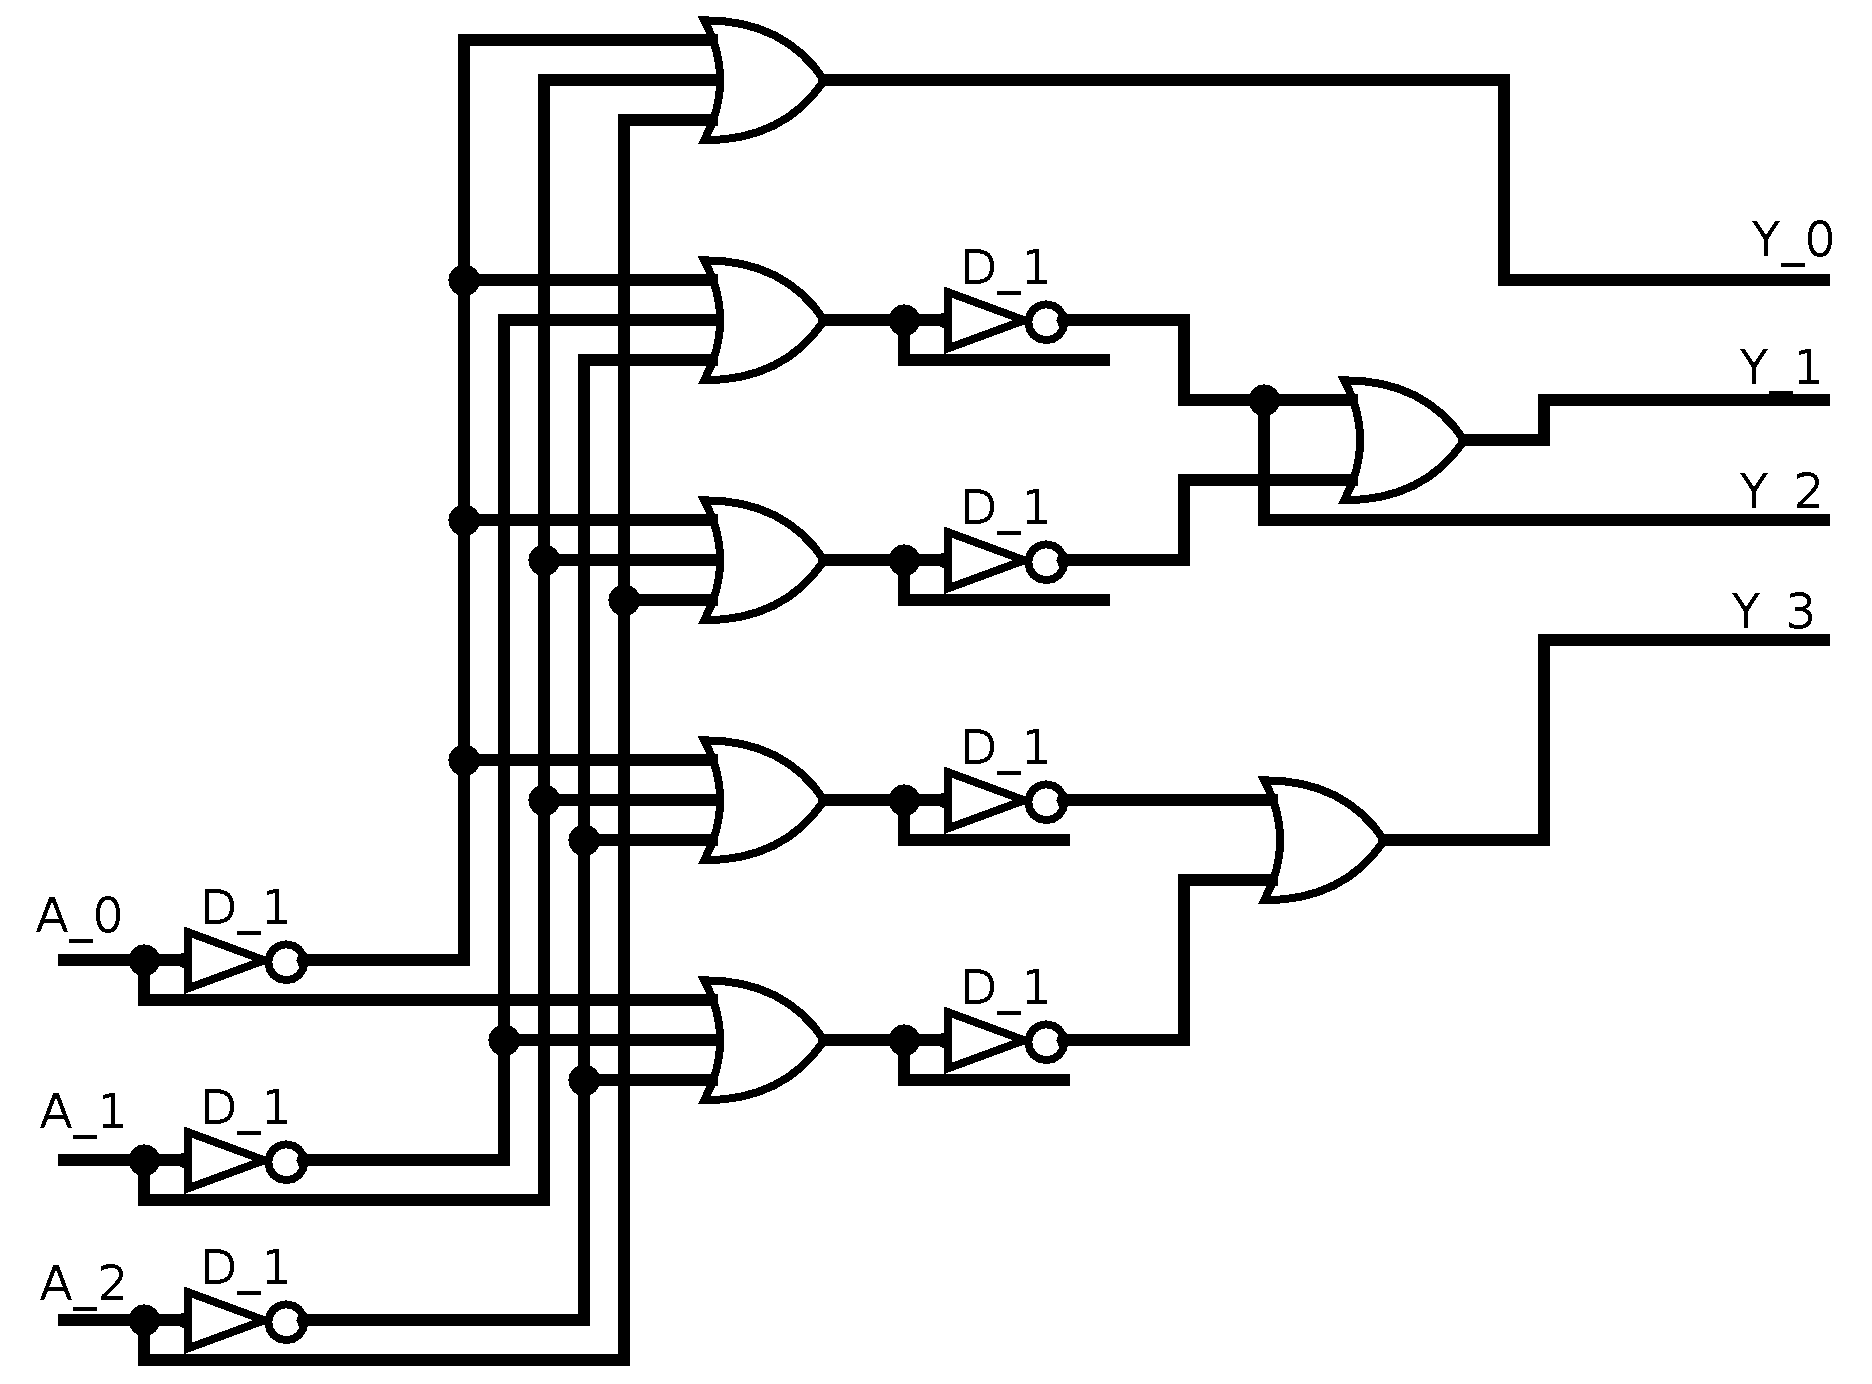
\includegraphics[width=14cm]{circuit_3.png}
        Datum: 12.11.1997, Funktion-ON-Mengen: \\
        $Y_0 = A_0' + A_1 + A_2$ \\
        $Y_1 = A_0A_1'A_2' + A_0A_1A_2$ \\
        $Y_2 = A_0A_1A_2$ \\
        $Y_3 = A_0A_1'A_2 + A_0'A_1A_2$ \\
        Begr�ndung: Da ein $D_1$-Dekoder 'zuf�llig' die Negation mit ausgibt, und \\
        $(B \wedge C) = \neg(\neg B \vee \neg C)$ ist, verwendet Diese Schaltung nur 'ODER'-Gatter und
        $D_1$-Dekoder.
\end{itemize}

\section*{Aufgabe 4}
\begin{itemize}

    \item Beh.: $T(N)$ hat $N$ Bl�tter. \\
        Da das Ziel ist, einen Eingang (die Wurzel) $N$-fach zu vervielf�ltigen, und wir nur
        von einem Blatt ein Signal 'ausgeben' k�nnen (sowie unsere Struktur ein Baum ist),
        ist gegeben dass wir bei $N$ Ausg�ngen $N$ Bl�tter haben m�ssen. \hfill $\Box$

    \item Beh.: $T(N)$ hat $\leq N/9 + s$ innere Knoten. \\
        O.b.d.A.: $N \in \mathbb{N}$  (1,..) \\
        IA: $s = 0 \Leftrightarrow N \in \{10^{s-1} + 1,..., 10^s\} = N \in \{10^0 = 1\} = N = 1$. \\
        $T(1)$ hat $\leq N/9 + s = 1/9 + 0$ innere Knoten. Stimmt, da der Baum nur ein Blatt hat,
        das gleichzeitig die Wurzel ist. \\
        IS: ($s \rightarrow s + 1$) \\
        Wenn $N$ gro� genug wird, um $N \notin \{10^{s-1} + 1,..., 10^s\}$ zu sein, muss $s$
        vergr��ert werden ?

    \item Beh.: Alle Pfade von der Wurzel zu einem Blatt in $T(N)$ haben L�nge $s$. \\


\end{itemize}

\end{document}
